% ! TeX program = lualatex
\documentclass[a4paper,11pt]{article} 
% packages
\usepackage{censor}
\StopCensoring
\usepackage{fontspec}
\setmainfont{EB Garamond}
% for tironian et fallback
% % \directlua{luaotfload.add_fallback
% % ("emojifallback",
% %      {"Noto Serif:mode=harf"}
% % )}
% % \setmainfont{EB Garamond}[RawFeature={fallback=emojifallback}]

\setmonofont[Scale=MatchLowercase]{Deja Vu Sans Mono}
\usepackage[a4paper,left=2cm,right=2cm,top=\dimexpr15mm+1.5\baselineskip,bottom=2cm]{geometry}
\setlength{\parindent}{0pt}

\usepackage{fancyhdr}       % Headers and footers 
\fancyhead[R]{\normalfont \leftmark}
\fancyhead[L]{}
\pagestyle{fancy}

\usepackage{microtype}      % Slightly tweak font spacing for aesthetics
\usepackage[english]{babel} % Language hyphenation and typographical rules
\usepackage{xcolor}
\definecolor{linkblue}{RGB}{0, 64, 128}
\usepackage[final, colorlinks = false, urlcolor = linkblue]{hyperref} 
% \newcommand{\secref}[1]{\textbf{§~\nameref{#1}}}
\newcommand{\secref}[1]{\textbf{§\ref{#1}~\nameref{#1}}}

\usepackage{changepage}     % adjust margins on the fly
\usepackage{amsmath,amssymb}

\usepackage{minted}
\usemintedstyle{algol_nu}

\usepackage{pgfplots}
\pgfplotsset{width=\textwidth,compat=1.9}

\usepackage{caption}
\newenvironment{code}{\captionsetup{type=listing}}{}
\captionsetup[listing]{skip=0pt}
\setlength{\abovecaptionskip}{5pt}
\setlength{\belowcaptionskip}{5pt}

\usepackage[yyyymmdd]{datetime}
\renewcommand{\dateseparator}{--}

\usepackage{enumitem}

\usepackage{titlesec}

\author{Andrew Hayes}

\begin{document}
\begin{titlepage}
    \begin{center}
        \hrule
        \vspace*{0.6cm}
        \Huge \textsc{ct414}
        \vspace*{0.6cm}
        \hrule
        \LARGE
       \vspace{0.5cm}
       Distributed Systems \& Co-Operative Computing
       \vspace{0.5cm}
       \hrule

       \vfill

       \hrule
        \begin{minipage}{0.495\textwidth} 
            \vspace{0.4em}
            \raggedright
            \normalsize 
            \begin{tabular}{@{}l l}
                Name: & Andrew Hayes \\
                Student ID: & 21321503 \\
                E-mail: & \href{mailto://a.hayes18@universityofgalway.ie}{a.hayes18@universityofgalway.ie} \\
            \end{tabular}
        \end{minipage}
        \begin{minipage}{0.495\textwidth} 
            \raggedleft
            \vspace*{0.8cm}
            \Large
            \today
            \vspace*{0.6cm}
        \end{minipage}
        \medskip\hrule 
    \end{center}
\end{titlepage}

\pagenumbering{roman}
\newpage
\tableofcontents
\newpage
\setcounter{page}{1}
\pagenumbering{arabic}

\section{Introduction}
\subsection{Client-Server Architectures}
\subsubsection{Two-Tier Architectures}
A \textbf{two-tier client-server architecture} is a client-server architecture wherein a client talks directly to a server, with no intervening server.
It is typically used in small environments ($\lesssim$ 50 users).
\\\\
A common development error is to prototype an application in a small, two-tier environment, and then scale up by simply adding more users to the server:
this approach will usually result in an ineffective system, as the server becomes overwhelmed.
To properly scale to hundreds or thousands of users, it is usually necessary to move to a three-tier architecture.

\begin{figure}[H]
    \centering
    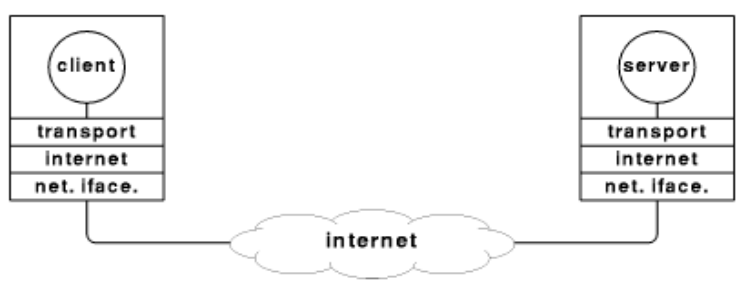
\includegraphics[width=0.7\textwidth]{./images/client-server-tcpip.png}
    \caption{
        Client \& server using TCP/IP protocols to communicate.
        Information can flow in either or both directions.
        The client \& server can interact with a transport layer protocols.
    }
\end{figure}

\subsection{Three-Tier Architecture}
A \textbf{three-tier client-server architecture} introduces a server or \textbf{agent} (or \textbf{load-balancer}) between the client \& the server.
The agent has many roles:
\begin{itemize}
    \item   Translation services: such as adapting a legacy application on a mainframe to a client-server environment.
    \item   Metering services: such as acting as a transaction monitor to limit the number of simultaneous requests to a given server.
    \item   Intelligent agent services: as in mapping a request to a number of different servers, collating the results, and returning a single response to the client.
\end{itemize}

\subsection{Network Programming Paradigms}
Practically all network programming is based on a client-server model; the only real difference in paradigms is the \textbf{level} at which the programmer operates.
The sockets API provides direct access to the available transport layer protocols.
RPC is a higher-level abstraction that hides some of the lower-level complexities.
Other approaches are also possible:
\begin{itemize}
    \item   Sockets are probably the best-known and most widely-used paradigm.
            However, problems of data incompatibility across platforms can arise.

    \item   RPC libraries aim to solve some of the basic problems with sockets and provide a level of transport independence.

    \item   Neither approach works very well with modern applications (Java RMI and other mdoern technologies, e.g., web services are better).
\end{itemize}

\section{Java RMI}
\textbf{Remote Method Invocation (RMI)} is a Java-based mechanism for distributed object computing.
RMI enables the distribution of work to other Java objects residing in other processes or on other machines.
The objects in one Java Virtual Machine (JVM) are allowed to seamlessly invoke methods on objects in a remote JVM.
To call a method of a remote object, we must first get a reference to that object, which can be obtained from  the registry name facility or by receiving the reference as an argument or return value of a method call.
Clients can call a remote object in a server that itself is a client of another server.
Parameters of method calls are passed as serialised objects: 
\begin{itemize}
    \item   types are not truncated, and therefore, object-oriented polymorphism is supported;
    \item   parameters are passed by value (deep copy) and therefore object behaviour can be passed.
\end{itemize}















\end{document}
